% !TEX program = xelatex
% !TEX root = main.tex

\documentclass[12pt, a4paper]{article}

\usepackage{fontspec}
\setmainfont[Ligatures=TeX]{Linux Libertine O}

\usepackage[hidelinks, colorlinks = true, urlcolor = blue]{hyperref}
\usepackage{indentfirst}

\usepackage{graphicx}
\graphicspath{{assets/}}

\usepackage[left=1.5cm,right=1.5cm,top=1.5cm,bottom=1.5cm]{geometry}
\usepackage{lipsum}

\usepackage[center]{caption}

\usepackage{subcaption}
\usepackage{dirtytalk}
\usepackage[final]{pdfpages}
\usepackage{cancel}
\usepackage{amsmath}
\usepackage{amssymb}
\usepackage{derivative}


\usepackage{hyperref}
\hypersetup{colorlinks = true, linkcolor = blue, }

\renewcommand{\figurename}{Εικόνα}
\setcounter{secnumdepth}{0}

%\setlength{\parindent}{1em}
\setlength{\parskip}{0.8em}

\title{\textbf{Ενσωματωμένα συστήματα πραγματικού χρόνου \\ \vspace{0.5cm} \normalsize{Τελικό Project - Συλλογή δεδομένων για χρηματοοικονομικά μέσα}}}
\author{
Θεόδωρος Κατζάλης \\
ΑΕΜ: 9282 \\
\texttt{katzalis@ece.auth.gr}
}
\date{Ιούνιος 2024}

\begin{document}

\sloppy
%\input{titlepage}
\maketitle

% {
% \renewcommand*\contentsname{Περιεχόμενα}
% \hypersetup{linkcolor=black}
% \tableofcontents
% }

%\pagebreak


\section{Εισαγωγή}

Η εργασία πραγματεύεται την ασύγχρονη συλλογή πληροφορίας συναλλαγών για σύμβολα από την πλατφόρμα finnhub. Τα σύμβολα που μελετήσαμε είναι AMZN, MSFT, BINANCE:USDT, και IC MARKETS: 1.

Η υλοποίηση αποσκοπεί στην αδιάκοπη λειτουργία του προγράμματος σε ένα ενσωματωμένο σύστημα, χρησιμοποιώντας παράλληλα νήματα και πιο συγκεκριμένα βασιζόμενοι στο μοντέλο συγχρονισμού producer-consumer.

Οι λειτουργίες που μας απασχολούν είναι:

%Έτσι χρησιμοποιήσαμε μια κοινή ουρά, στην οποία αποθηκεύαμε τις συναλλαγές που δεχόμασταν απο το finhub. Οι producers ήταν υπεύθυνοι για την προσθήκη αυτών των συναλλαγών και οι consumers για την επιτέλεση συγκεκριμένων λειτουργιών:
\vspace{-1em}
\begin{itemize}
\itemsep 0em
\item Καταγραφή συναλλαγών
\item Υπολογισμός candlestick για κάθε λεπτό, στο λεπτό
\item Υπολογισμός κινητού μέσου όρου των τιμών (price) των συμβόλων για τα πιο πρόσφατα 15 λεπτά
\end{itemize}
Καθένα απο τα παραπάνω αποθηκεύεται σε αρχείο ξεχωριστό για το κάθε σύμβολο. Το πρόγραμμα υλοποιήθηκε σε C, με pthreads για παραλληλοποίηση και με την χρήση της βιβλιοθήκης libwebsocket για την δημιουργία websocket ως το αμφίδρομο κανάλι επικοινωνίας με την πλατφόρμα finnhub.

Η εργασία και ο κώδικας μπορούν να βρεθούν σε αυτό το αποθετήριο \url{https://github.com/thodkatz/embedded-rtos}. Ο φάκελος \verb|producer_consumer| περιέχει ένα πρότυπο πρόβλημα producer-consumer (preparatory homework), και ο φάκελος \verb|finnhub| την συγκεκριμένη εργασία, βασιζόμενοι σε αυτό το πρότυπο. Το πρόγραμμα είχε χρόνο εκτέλεσης 50:46:18.77 (hh:mm:ss).


\section{Μεθοδολογία}

Πρωταρχικό στάδιο ήταν η υλοποίηση ενός finnhub client με websocket, και η επιτυχής λήψη συναλλαγών. Αρχικά, μέσω του websocket στείλαμε μηνύματα εγγραφής στα σύμβολα που μας απασχολούν, όπως ορίζεται και από το API documentation (π.χ \verb|'{"type":"subscribe-news","symbol":"AAPL"}'|), και στη συνέχεια λαμβάναμε την πληροφορία των συναλλαγών με callback συναρτήσεις. Η αφετηρία της λήψης πληροφορίων γίνεται με την κλήση της \verb|lws_service()|, υπεύθυνη για την διαχείριση των events.

Αυτό που θα μας απασχολήσει περισσότερο είναι η τεχνική παραλληλοποίησης του προβλήματος. Όπως αναφέρθηκε προηγουμένως, η προσέγγιση μας βασίζεται στο πρόβλημα producer-consumer. Οι producers είναι υπεύθυνοι να περιμένουν και να προσθέτουν την πληροφορία των events (\verb|queueAdd()|) σε μια κοινή ουρά. Οι consumers, σε πραγματικό χρόνο, καταναλώνουν τα δεδομένα απο την ουρά (\verb|queueDel()|), καταγράφοντας σε αρχείο τις συναλλαγές, και υπολογίζοντας τις αθροιστικές τιμές για candlesticks και για τον κινητό μέσο όρο.

Για την καταγραφή των candlesticks στο λεπτό και του κινητού μέσου όρου, έχουμε ένα ξεχωριστό νήμα, τον scheduler. Αυτό παραμένει αδρανές για ένα λεπτό, μέχρι οι producers και οι consumers να συλλέξουν και επεξεργαστούν τα δεδομένα, και στη συνέχεια αποθηκεύει τους υπολογισμούς σε αρχεία. Όλα τα νήματα ασχολούνται με κοινούς πόρους και για την επίτευξη συνοχής διαμοιράζονται ένα mutex. Έτσι, οταν καλείται ο scheduler και γίνεται κάτοχος του κλειδιού (η κοινή ουρά παύει να υφίσταται οποιαδήποτε επεξεργασία απο τους producers και consumers), καταγράφουμε σε αρχεία τις πληροφορίες που συλλέχθηκαν στο μεσοδιάστημα, και αρχικοποιούνται οι δομές δεδομένων (\verb|struct candlestickMinute|) υπεύθυνες για τους υπολογισμούς του ενός λεπτού.

Ο scheduler ακόμη, αποθηκεύει την μέση τιμή της τιμής (price) των συναλλαγών, κατά τη διάρκεια ενός λεπτού ως την τιμή του λεπτού, στην δομή δεδομένων που είναι υπεύθυνη για τον υπολογισμό του κινητού μέσου όρου (\verb|struct movingAverage|), που αποτελείται απο μια λίστα 15 στοιχείων, των πιο πρόσφατων λεπτών.

Επομένως υπάρχουν αλληλεξαρτήσεις στα νήματα που έχουμε αναφέρει. Οι producers προσθέτουν στην ουρά, οι consumers αφαιρούν απο την ουρά, και ο scheduler "παγώνει" την επεξεργασία πληροφορίας για να καταγράψει την κατάσταση του λεπτού. Ενδιαφέρον παρουσιάζει, η καθυστέρηση του scheduler εξαιτίας του mutex, και του ανταγωνισμού με τα υπόλοιπα νήματα στο να αποκτήσει το κλειδί. Για να αυξήσουμε την ακρίβεια ως προς τον χρόνο, για την καταγραφή των δεδομένων, θα μπορούσαμε να θέσουμε το νήμα του scheduler με την υψηλότερη προτεραιότητα, αλλά θα έπρεπε να εξεταστεί και η επεξεργασία των εναπομείναντων δεδομένων της κοινής ουράς από τους consumers. Οπότε η βέλτιστη πολιτική προτεραιότητας θα ήταν κατά την κλήση του scheduler, να "παγώνουν" οι producers, να αδειάζουν την ουρά οι consumers, και ύστερα να γίνεται η καταγραφή.

Η παραπάνω διαπίστωση έγινε σε μεταγενέστερο στάδιο και τα αποτελέσματα μας ακολουθούν μια πιο απλή μεθοδολογία, όπου όλα τα νήματα έχουν την ίδια προτεραιότητα, και ο scheduler, όταν καλείται, μετά την απόκτηση του κλειδιού, καταγράφει την πληροφορία χωρίς κάποια συνθήκη. Το μειονέκτημα είναι ότι υπάρχει η πιθανότητα να μην συμπεριλάβουμε στους υπολογισμούς κάποιες συναλλαγές, που ανήκουν στο τρέχων λεπτό, και δεν έχουν επεξεργαστεί απο τους consumers όταν κλήθηκε ο scheduler. Ωστόσο η πληροφορία δεν χάνεται και προσμετράται για το επόμενο λεπτό, στην επόμενη κλήση του scheduler.

Για την εξασφάλιση της αδιάκοπης λειτουργίας, οι producers είναι υπεύθυνοι για την επανασύνδεση με το websocket, και το πρόγραμμα τερματίζει με την αποστολή σήματος SIGINT.

Αξίζει να σημειωθεί ότι χρησιμοποιήθηκαν 2 νήματα για producers, 2 για consumers, και 1 scheduler. Το μέγεθος της κοινής ουράς ήταν 100 στοιχείων. Η μελέτη για την επίδραση της ουράς, και τον αριθμό των νημάτων έχει γίνει στο prepatory homework, του οποίου την αναφορά μπορείτε να δείτε \href{https://github.com/thodkatz/embedded-rtos/blob/master/producer_consumer/report.pdf}{εδώ}.


\section{Αποτελέσματα}

Παρακάτω παραθέτουμε τα αποτελέσματά του προγράμματος. Μπορούμε να δούμε την α) πορεία των candlesticks, β) τον κινητό μέσο όρο της τιμής των συμβόλων για τα 15 πιο πρόσφατα λεπτά, και γ) το χρόνο που μεσολάβησε μεταξύ του χρόνου καταγραφής της συναλλαγής με την χρονική στιγμή της συναλλαγής που παρέχεται ως πεδίο των δεδομένων του finhhub. Ακόμη, για να δούμε πόσο αποκλίνει ο scheduler απο το λεπτό, όπως αναφέρθηκε προηγουμένως ορίσαμε ως ποσοστιαία απόκλιση του scheduler:
$\frac{\text{Χρονική στιγμή καταγραφής scheduler} - (\text{Προηγούμενη χρονική στιγμή καταγραφής scheduler} + 1 \text{ λεπτό})}{1 \text{ λεπτό}}$

\begin{figure}[h!]
\centering
\begin{subfigure}[b]{0.45\textwidth}
\centering
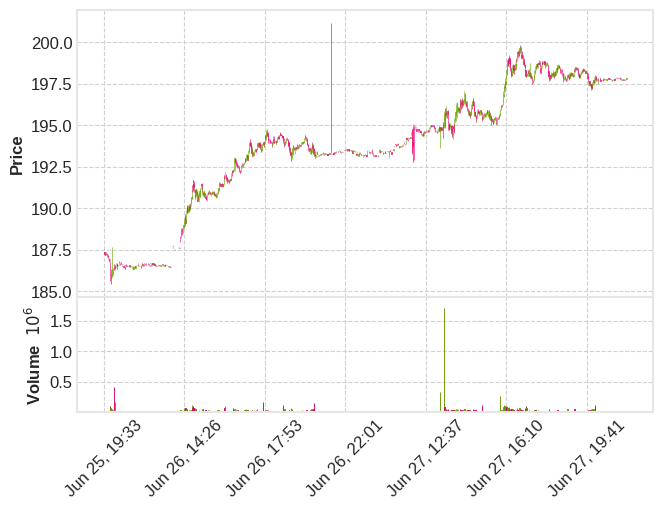
\includegraphics[width=\textwidth]{amzn_candlesticks.png}
\caption{Candlesticks}
\label{fig:sub1}
\end{subfigure}
\hfill
\begin{subfigure}[b]{0.45\textwidth}
\centering
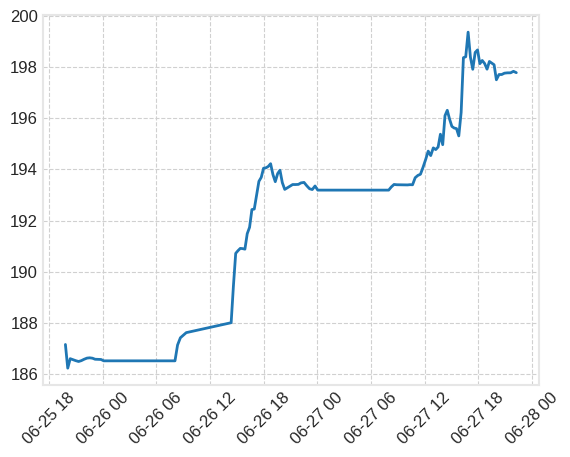
\includegraphics[width=\textwidth]{amzn_ma.png}
\caption{Κινητός μέσος όρος τιμής 15 πιο πρόσφατων λεπτών}
\label{fig:sub2}
\end{subfigure}

\vskip\baselineskip

\begin{subfigure}[b]{0.45\textwidth}
\centering
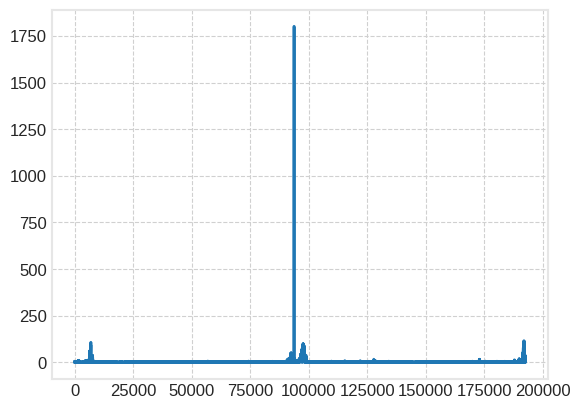
\includegraphics[width=\textwidth]{delay_transactions_line.png}
\caption{Χρονική καθυστέρηση καταγραφής συναλλαγών (s)}
\label{fig:sub3}
\end{subfigure}
\hfill
\begin{subfigure}[b]{0.45\textwidth}
\centering
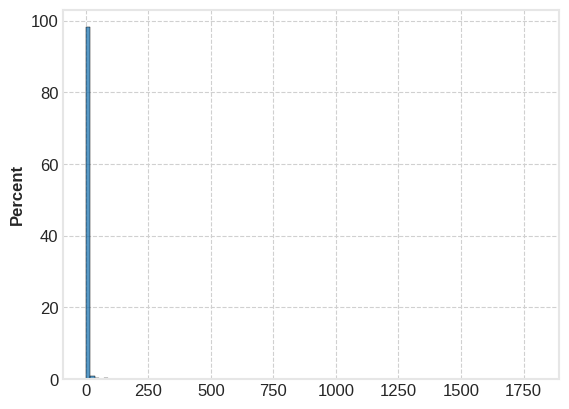
\includegraphics[width=\textwidth]{delay_transactions_hist.png}
\caption{Ιστόγραμμα χρονικής καθυστέρησης καταγραφής συναλλαγών (s)}
\end{subfigure}

\vskip\baselineskip

\begin{subfigure}[b]{0.45\textwidth}
\centering
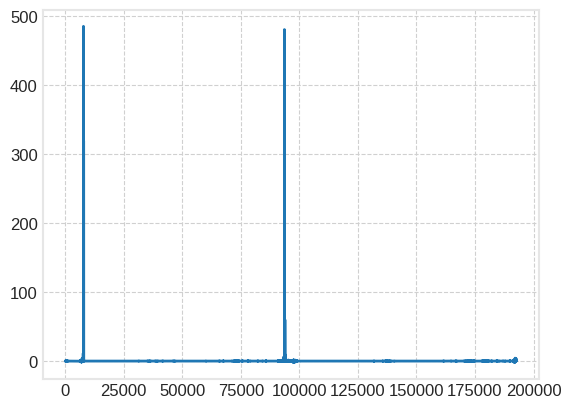
\includegraphics[width=\textwidth]{delay_candlestick_line.png}
\caption{Ποσοστιαία απόκλιση του λεπτού του scheduler}
\label{fig:sub3}
\end{subfigure}
\hfill
\begin{subfigure}[b]{0.45\textwidth}
\centering
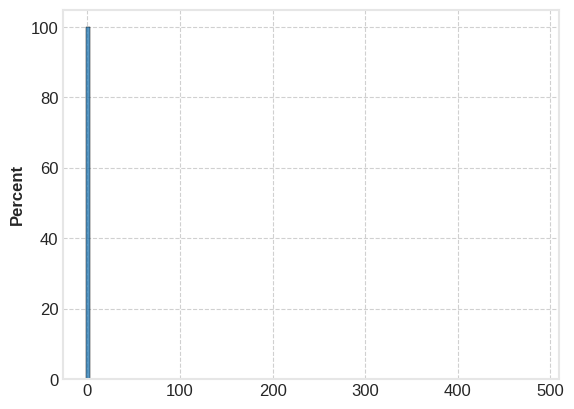
\includegraphics[width=\textwidth]{delay_candlestick_hist.png}
\caption{Ιστόγραμμα ποσοστιαίας απόκλισης του λεπτού του scheduler}
\end{subfigure}
\caption{AMZN}
\end{figure}

\begin{figure}[h!]
\centering
\begin{subfigure}[b]{0.45\textwidth}
\centering
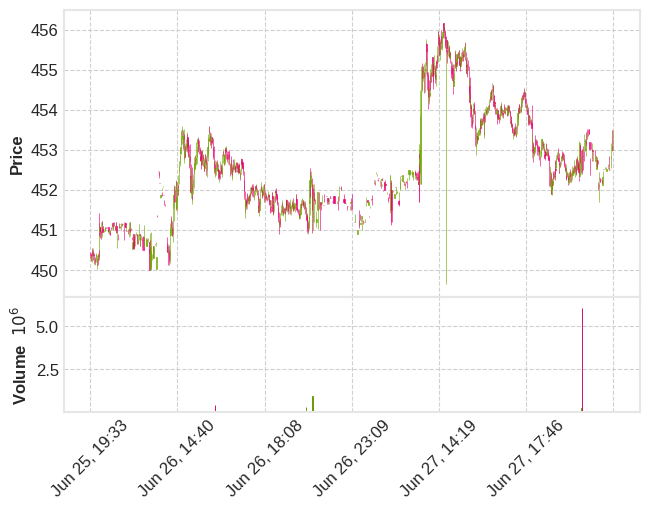
\includegraphics[width=\textwidth]{msft_candlesticks.png}
\caption{Candlesticks}
\label{fig:sub1}
\end{subfigure}
\hfill
\begin{subfigure}[b]{0.45\textwidth}
\centering
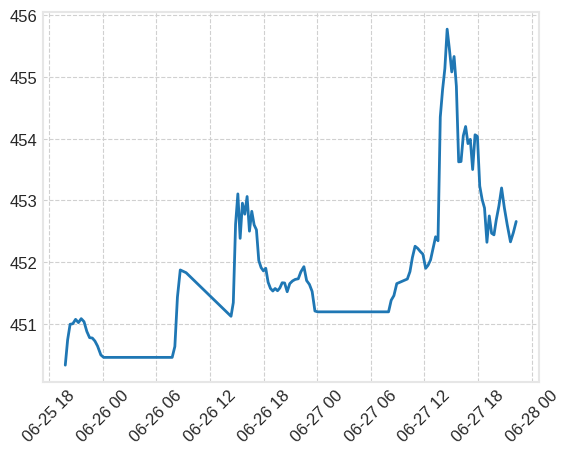
\includegraphics[width=\textwidth]{msft_ma.png}
\caption{Κινητός μέσος όρος τιμής 15 πιο πρόσφατων λεπτών}
\label{fig:sub2}
\end{subfigure}

\vskip\baselineskip

\begin{subfigure}[b]{0.45\textwidth}
\centering
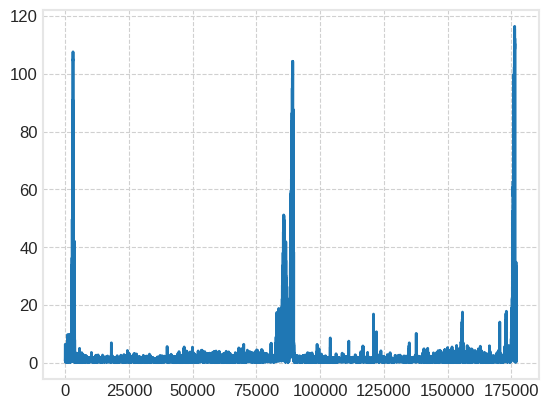
\includegraphics[width=\textwidth]{delay_transactions_line_msft.png}
\caption{Χρονική καθυστέρηση καταγραφής συναλλαγών (s)}
\label{fig:sub3}
\end{subfigure}
\hfill
\begin{subfigure}[b]{0.45\textwidth}
\centering
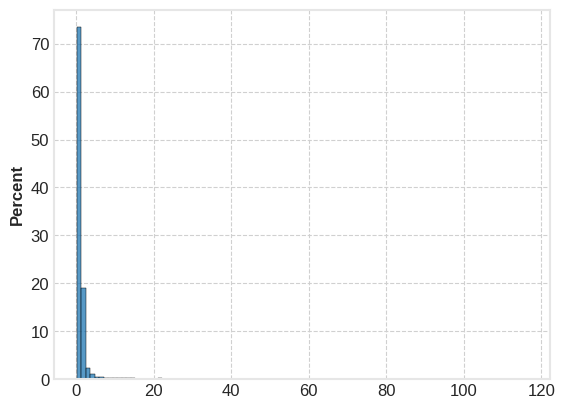
\includegraphics[width=\textwidth]{delay_transactions_hist_msft.png}
\caption{Ιστόγραμμα χρονικής καθυστέρησης καταγραφής συναλλαγών (s)}
\end{subfigure}

\vskip\baselineskip

\begin{subfigure}[b]{0.45\textwidth}
\centering
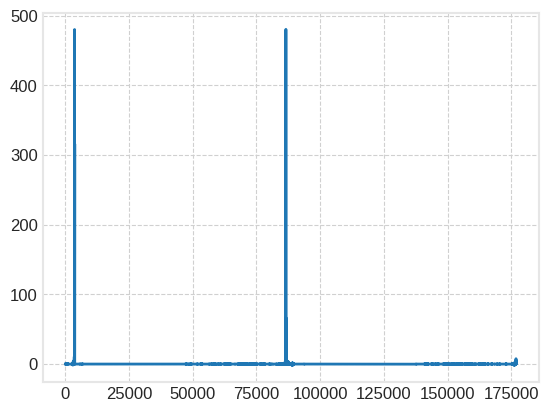
\includegraphics[width=\textwidth]{delay_candlestick_line_msft.png}
\caption{Ποσοστιαία απόκλιση του λεπτού του scheduler}
\label{fig:sub3}
\end{subfigure}
\hfill
\begin{subfigure}[b]{0.45\textwidth}
\centering
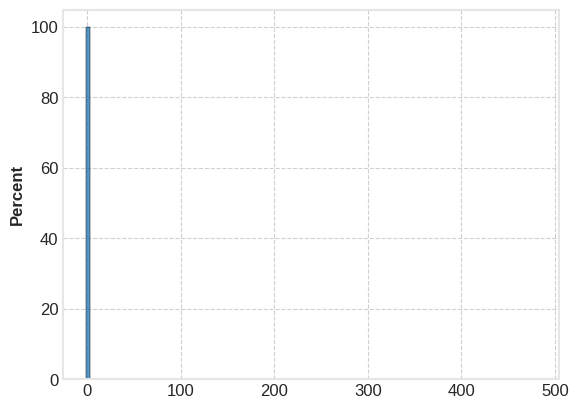
\includegraphics[width=\textwidth]{delay_candlestick_hist_msft.png}
\caption{Ιστόγραμμα ποσοστιαίας απόκλισης του λεπτού του scheduler}
\end{subfigure}
\caption{MSFT}
\end{figure}

\begin{figure}[h!]
\centering
\begin{subfigure}[b]{0.45\textwidth}
\centering
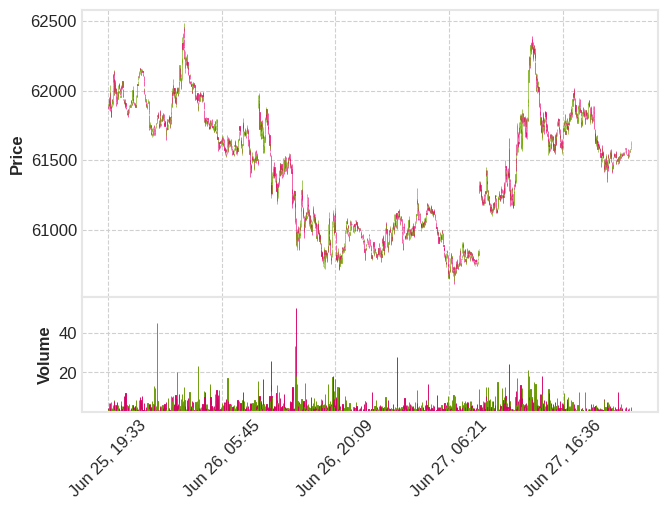
\includegraphics[width=\textwidth]{binance_candlesticks.png}
\caption{Candlesticks}
\label{fig:sub1}
\end{subfigure}
\hfill
\begin{subfigure}[b]{0.45\textwidth}
\centering
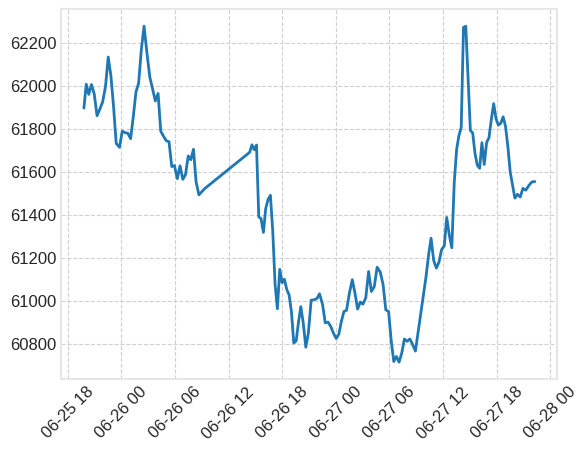
\includegraphics[width=\textwidth]{binance_ma.png}
\caption{Κινητός μέσος όρος τιμής 15 πιο πρόσφατων λεπτών}
\label{fig:sub2}
\end{subfigure}

\vskip\baselineskip

\begin{subfigure}[b]{0.45\textwidth}
\centering
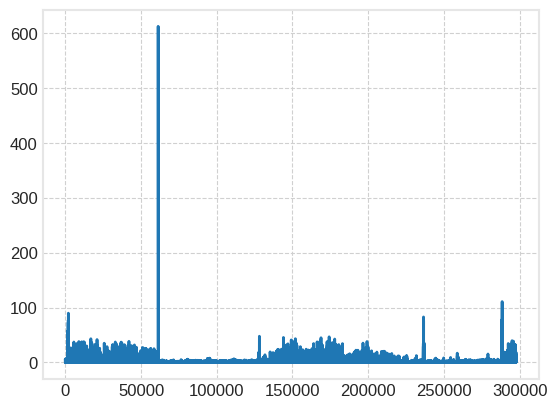
\includegraphics[width=\textwidth]{delay_transactions_line_binance.png}
\caption{Χρονική καθυστέρηση καταγραφής συναλλαγών (s)}
\label{fig:sub3}
\end{subfigure}
\hfill
\begin{subfigure}[b]{0.45\textwidth}
\centering
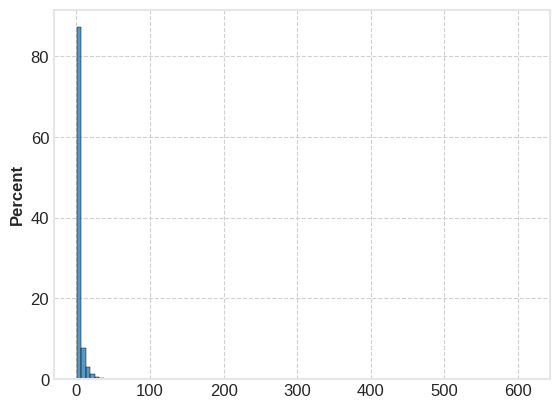
\includegraphics[width=\textwidth]{delay_transactions_hist_binance.png}
\caption{Ιστόγραμμα χρονικής καθυστέρησης καταγραφής συναλλαγών (s)}
\end{subfigure}

\vskip\baselineskip

\begin{subfigure}[b]{0.45\textwidth}
\centering
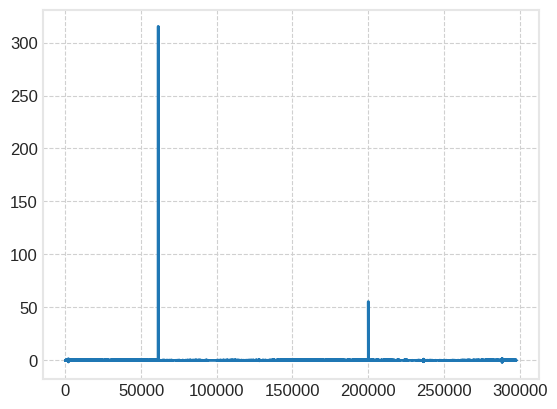
\includegraphics[width=\textwidth]{delay_candlestick_line_binance.png}
\caption{Ποσοστιαία απόκλιση του λεπτού του scheduler}
\label{fig:sub3}
\end{subfigure}
\hfill
\begin{subfigure}[b]{0.45\textwidth}
\centering
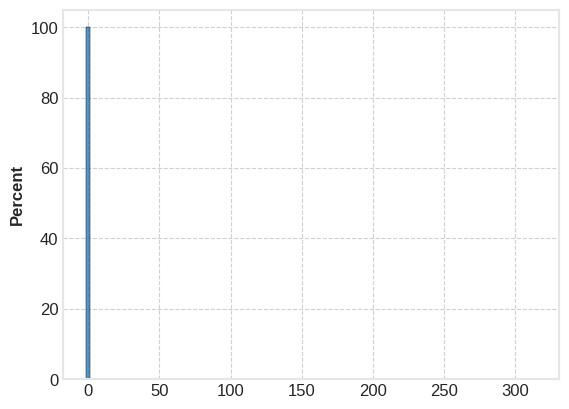
\includegraphics[width=\textwidth]{delay_candlestick_hist_binance.png}
\caption{Ιστόγραμμα ποσοστιαίας απόκλισης του λεπτού του scheduler}
\end{subfigure}
\caption{Binance}
\end{figure}

\begin{figure}[h!]
\centering
\begin{subfigure}[b]{0.45\textwidth}
\centering
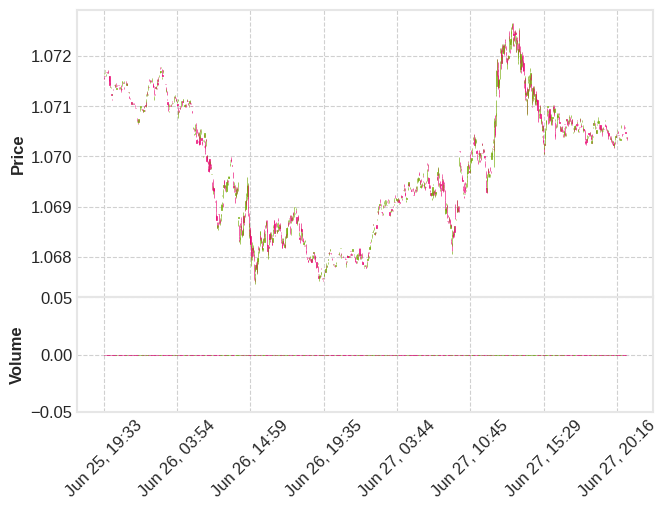
\includegraphics[width=\textwidth]{icm_candlesticks.png}
\caption{Candlesticks}
\label{fig:sub1}
\end{subfigure}
\hfill
\begin{subfigure}[b]{0.45\textwidth}
\centering
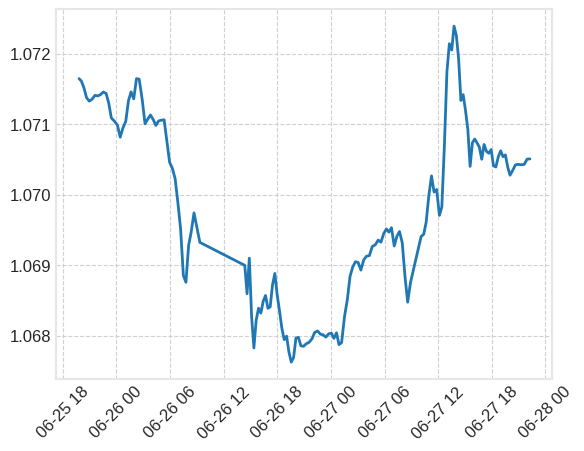
\includegraphics[width=\textwidth]{icm_ma.png}
\caption{Κινητός μέσος όρος τιμής 15 πιο πρόσφατων λεπτών}
\label{fig:sub2}
\end{subfigure}

\vskip\baselineskip

\begin{subfigure}[b]{0.45\textwidth}
\centering
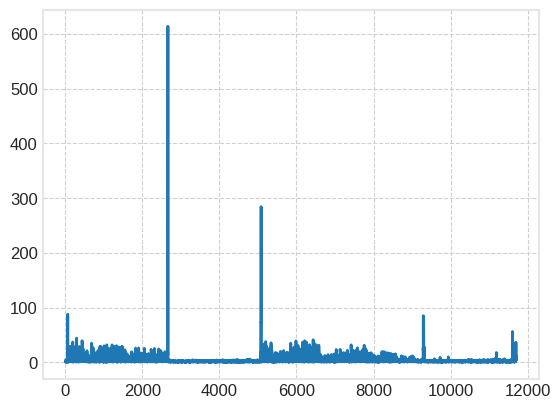
\includegraphics[width=\textwidth]{delay_transactions_line_icm.png}
\caption{Χρονική καθυστέρηση καταγραφής συναλλαγών (s)}
\label{fig:sub3}
\end{subfigure}
\hfill
\begin{subfigure}[b]{0.45\textwidth}
\centering
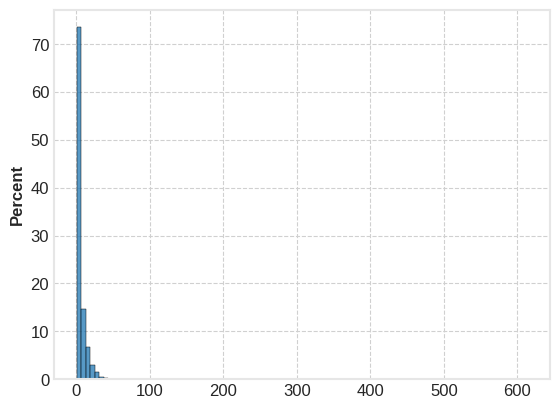
\includegraphics[width=\textwidth]{delay_transactions_hist_icm.png}
\caption{Ιστόγραμμα χρονικής καθυστέρησης καταγραφής συναλλαγών (s)}
\end{subfigure}

\vskip\baselineskip

\begin{subfigure}[b]{0.45\textwidth}
\centering
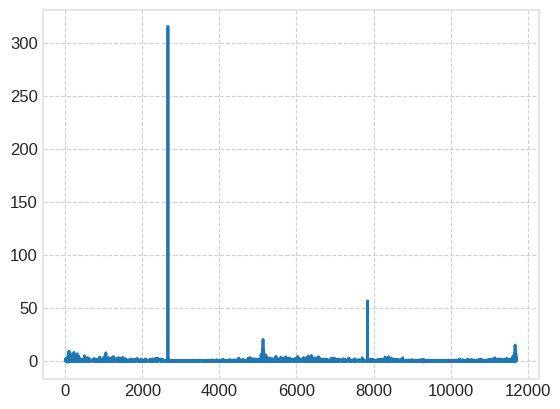
\includegraphics[width=\textwidth]{delay_candlestick_line_icm.png}
\caption{Ποσοστιαία απόκλιση του λεπτού του scheduler}
\label{fig:sub3}
\end{subfigure}
\hfill
\begin{subfigure}[b]{0.45\textwidth}
\centering
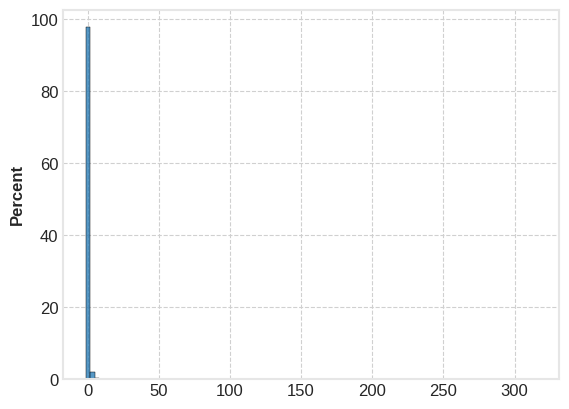
\includegraphics[width=\textwidth]{delay_candlestick_hist_icm.png}
\caption{Ιστόγραμμα ποσοστιαίας απόκλισης του λεπτού του scheduler}
\end{subfigure}
\caption{IC MARKETS: 1}
\end{figure}

\clearpage

Για να καταγράψουμε πόσο χρόνο η CPU μένει αδρανής, χρησιμοποιήσαμε την εντολή \verb|time|, με το ακόλουθο αποτέλεσμα:

\verb|./bin/client 132.68s user 38.90s system 0% cpu 50:46:18.77 total|


\section{Συμπεράσματα}

\begin{itemize}
\itemsep 0em
\item Υπήρχαν κάποια χρονικά διαστήματα που δεν λαμβάναμε πληροφορία για συναλλαγές. Αυτό οφείλεται στην λειτουργία της πλατφόρμας finnhub, και όχι στην δική μας υλοποίηση. Εκεί παρατηρούμε κενά στα διαγράμματα candlesticks.
\item Στις χρονικές στιγμές που χανόταν η σύνδεση, και ένας από τους producers προσπαθούσε για επανασύνδεση, παρατηρούμε μεγάλες χρονικές καθυστερήσεις στα διαγράμματα χρόνου. Αυτό οφείλεται επειδή οι consumers και ο scheduler, περιμένουν να τελειώσουν την δουλειά τους οι producers, υπεύθυνοι για την επανασύνδεση, που ενδεχομένως να απαιτεί αρκετές χρονοβόρες προσπάθειες.
\item Από το αποτέλεσμα της εντολής \verb|time|, συμπεραίνουμε ότι το πρόβλημα είναι I/O bound και όχι CPU bound, μιας και η CPU την περισσότερη ώρα βρίσκεται σε αναμονή.
\end{itemize}

\end{document}
